Quindi grazie a quanto illustrato finora abbiamo verificato che data una lunghezza fissata il periodo di oscillazione del pendolo non dipende dalla massa applicata ad esso. Inoltre possiamo dire che non c'è stata nemmeno un deformazione apprezzabile del filo utilizzato in quanto tutte le misure effettuate risultano compatibili con i valori ottenuti.

La non dipendenza del periodo dalla massa si può anche ricavare grazie ad un analisi dimensionale; ovvero: se suponiamo che il periodo del pendolo $\mathcal{T}$ possa dipendere dalla massa appesa $m$, dalla lunghezza del filo $\ell$ e dall'accelerazione di gravità $g$ mediante una relazione del tipo $\mathcal{T} \,\propto\, m^\alpha \, \ell^\beta \, g^\gamma$.\\
Studiando le dimensioni di $\mathcal{T}, \,\, m, \,\, \ell \,\,e\,\, g$ si ottiene che l'equazione dimensionale corretta è la seguente:

\begin{equation*}
	[T]^1 \,=\, [M]^\alpha[L]^{\beta+\gamma}[T]^-2\gamma 
\end{equation*}
%
che risulta essere soddisfatta per

\begin{equation*}
	\alpha \,=\, 0; \quad \gamma \,=\, -1/2; \quad \beta \,=\, -\gamma \,=\, 1/2 
\end{equation*}
%
da cui abbiamo che:

\begin{equation*}
	\mathcal{T} \,=\, \mathcal{C} \, \sqrt{\frac{\ell}{g}}
\end{equation*}
%
dove il parametro $\mathcal{C}$ è una costante il cui valore non si può determinare dal semplice calcolo dimensionale. Si nota che poichè risulta essere necessario che $\alpha$ sia uguale a 0 allora anche grazie ad un'analisi dimensionale abbiamo ottenuto una conferma che effettivamente il periodo di oscillazione di un pendolo non dipende dalla massa applicata.

\begin{SCfigure}
    \centering
    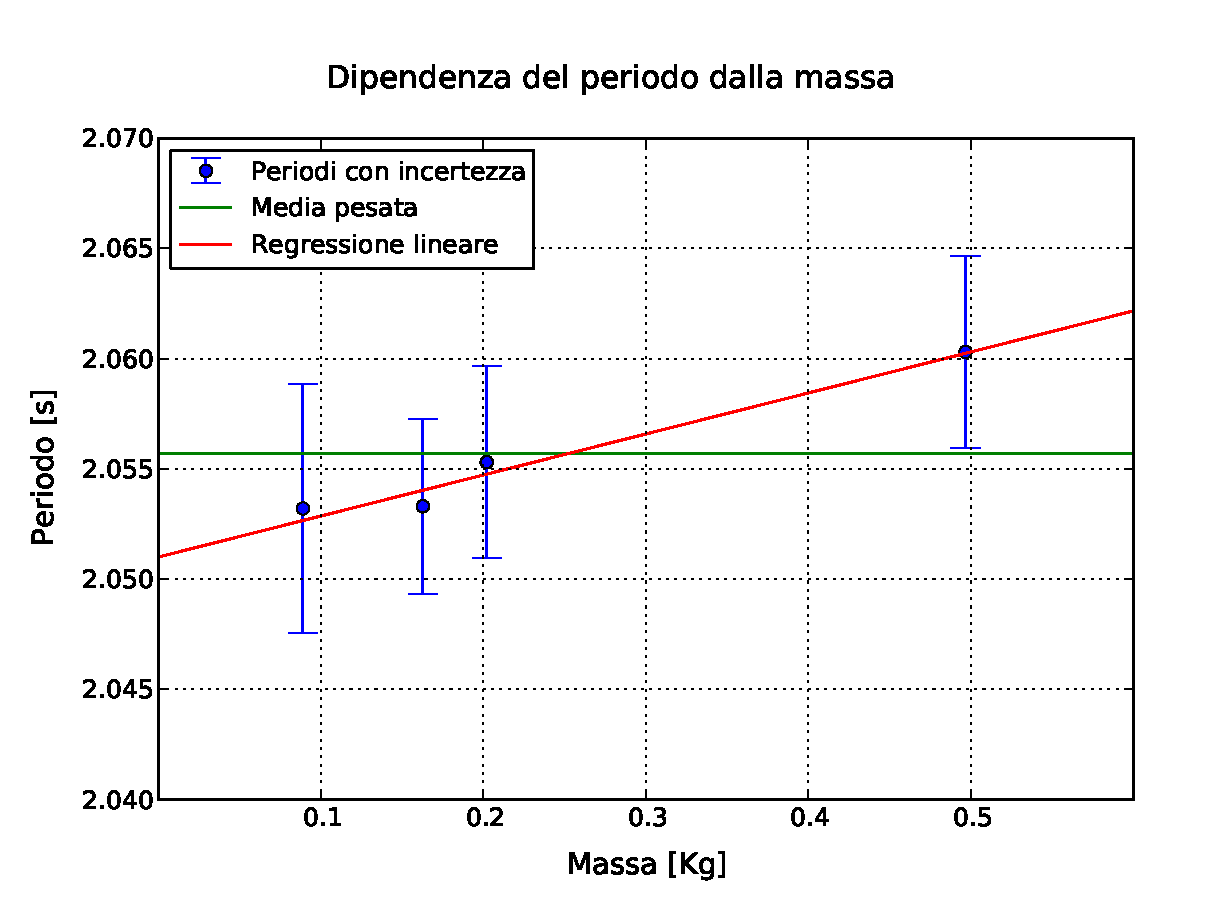
\includegraphics[width=120mm]{immagini/masse.pdf}
    \caption{Il seguente grafico rappresenta sull'asse delle ordinate le medie dei periodi relativi ad ogni singola massa, mentre sull'asse delle ascisse sono riportate le masse utilizate. L'incertezza sul periodo è differente da misura a misure, mentre quella reativa alla massa è uguele per tutte, ed in particolare è l'incertezza tipo. Il grafico inoltre con la retta orizzontale verde rappresenta il valore costante della media pesata delle medie dei periodi ($\mathcal{T}$), mentre in rosso è rappresentata la retta derivante dalla regressione lineare reltiva alla funzione $f \,:=\, \mathcal{T} - A - B\,m$.}
    \label{fig: periodo vs masse}
\end{SCfigure}